\documentclass{article}
\usepackage{algorithm}
\usepackage{algpseudocodex}
\usepackage{graphicx}
\usepackage{amsmath}
\usepackage{xcolor}
\usepackage{listings}
\usepackage{hyperref}

\definecolor{codegreen}{rgb}{0,0.6,0}
\definecolor{codegray}{rgb}{0.5,0.5,0.5}
\definecolor{codepurple}{rgb}{0.58,0,0.82}
\definecolor{backcolour}{rgb}{0.95,0.95,0.92}

\lstdefinestyle{mystyle}{
    backgroundcolor=\color{backcolour},   
    commentstyle=\color{codegreen},
    keywordstyle=\color{magenta},
    numberstyle=\tiny\color{codegray},
    stringstyle=\color{codepurple},
    basicstyle=\ttfamily\footnotesize,
    breakatwhitespace=false,         
    breaklines=true,                 
    captionpos=b,                    
    keepspaces=true,                 
    numbers=left,                    
    numbersep=5pt,                  
    showspaces=false,                
    showstringspaces=false,
    showtabs=false,                  
    tabsize=2
}

\lstset{style=mystyle}

\title{CSEP590 : Applied Cryptography: Homework 3}
\author{Karuna Sagar Krishna}

\begin{document}
    \maketitle

    \section*{Task 1a}
    As mentioned in the question, the server only publishes the root hash reliably. So when the client downloads a file from the server, to validate the integrity of this downloaded file, it needs to somehow compare with the root hash published by the server. We also know that hash functions are one-way functions, so we need recompute the root hash starting with the downloaded file. Calculating the hash of the downloaded file is straightforward. We then follow the same procedure followed at the sever to compute the root hash. To do so, we need the server to send hashes from other nodes in the tree as shown below. In the below diagram, we consider the file downloaded is $F_4$ and the corresponding hash is marked green which is computed by the client. The other hash values that should be sent by the server is marked yellow.

    \begin{figure}[H]
        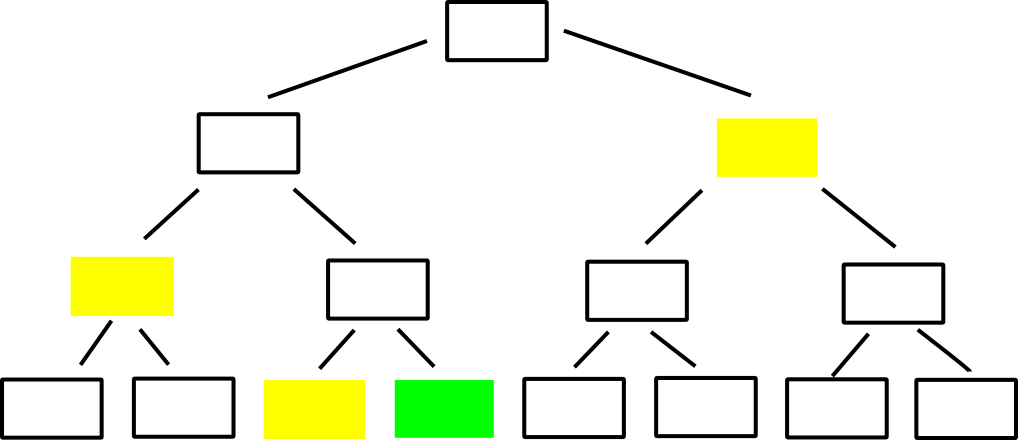
\includegraphics[width=1\textwidth]{completeBinaryTree.png}
    \end{figure}
    
    So, when the client requests the server to download any file $F_i$, the server should respond with the file contents and also the hashes (marked yellow above) required to recompute the root hash for integrity check. Here the server needs to send $\log m$ (where $m$ is the number of files hosted by the server) hashes along with the file contents. This is because the there are $m$ leaves and we are told that $m$ is a power of two. So we have a complete binary tree where the height of the tree is $\log m$.
    
    This is secure because any tampering to the file contents would lead a different hash of the file. This is due second pre-image and collision resistance properties of hash function. When we hash this with other hash values provided by the server, the difference of the hash propagates to the root. This can be detected since it won't match the root hash published reliably by the server. Further, it is possible for hashes sent by the server along with file contents to be tampered with. However, again this would be detected by a mismatch with published root hash due to second pre-image and collision resistance properties of hash function.

    \section*{Task 1b}
    The server would have change $\log m + 1$ hashes in total. First, the server has to recompute the hash of the changed file $F_i$ and then walk up the tree to update the root hash. Since the height of the tree is $\log m$ (as described above), the server has to perform $\log m$ operations to update each internal node and the root node. Finally, the server should publish this root hash reliably.

    \section*{Task 2a}
    Since we are using HMAC with SHA-256 to generate the MAC tag, we know that the resulting MAC is 256 bits long i.e. 32 bytes long. From $C_1$ and $C_2$ we see that the last 32 bytes are identical. Since we told that same keys were used to generate MACs, it indicates that the plain text must be the same. However, we see the cipher text is 50 bytes long and different between $C_1$ and $C_2$. Given that we are using CTR mode AES encryption, the first 16 bytes represents the initialization vector (IV). The IV for $C_1$ and $C_2$ are different which explains why the remaining cipher text blocks are different. We can also learn that the plain text is 34 bytes long i.e. 50 bytes - 16 bytes of IV. From class, we know that CTR mode AES offers IND-CPA security, so without the encryption key we cannot learn anything else about the plain text.

    \section*{Task 2b}
    Assuming the E\&M uses encryption scheme that provides IND-CPA security and MAC scheme that provides UF-CMA security notions. The cipher text resulting from E\&M has two parts - the cipher text output of the encryption scheme and the tag from MAC scheme. Clearly, the cipher text is IND-CPA secure but the MAC tag is not IND-CPA secure. An attacker/distinguisher can ask E\&M system to encrypt a chosen plain text twice; the encryption scheme would chose a random IV (or nonce) resulting in different cipher text, but the MAC scheme would return the same since it is based on the plain text. So the attacker can identify E\&M with a probability of one using 2 queries and linear time. However, an ideal truly random encryption scheme would return random cipher text. This leads a high advantage for the attacker to distinguish the E\&M system from a truly random system. Hence E\&M is not IND-CCA secure.

    \section*{Task 2c}
    INT-CTXT informally says that an attacker should not be able to modify the cipher text that leads to a valid decryption. In E\&M, the MAC tag is generated against the plain text. So clearly the UF-CMA notion is with respect to the plain text. Lets say we somehow know that Alice plans to send message "hello 590 students" to Bob using E\&M approach. Then an attacker could ask E\&M to encrypt "hello 591 students", extract the MAC tag, construct a new cipher text by flipping an appropriate bit in the cipher text and replacing the MAC tag with the extracted one. This new cipher text can be successfully decrypted by Bob. Note, this is not a copy attack since we are producing a cipher text not produced by E\&M system. Hence E\&M is not INT-CTXT secure.

    \section*{Task 3a}
    We can think of steps 1 and 2 in encryption algorithm as pre-processing step for plain text. In other words, after step 2, we have a new transformed plain text. Also, the original plain text is part of this transformed plain text along with additional bytes. This transformed plain text is encrypted using CTR mode that we studied in class. Hence we know that the output is IND-CPA secure with respect to the transformed plain text. Since the original plain text is a substring of this transformed plain text we can say IND-CPA security holds on the original plain text as well.

    \section*{Task 3b}
    As we saw in class, CTR mode offers no INT-CTXT security. Hence this scheme doesn't offer any cipher text integrity as well. It seems that $M[l+1]$ computed in step 2 of encryption algorithm roughly maps to a MAC tag. However, this does not offer UF-CMA since we can flip two bits from different message blocks at the same position which leads to the same $M[l+1]$ value but the original message is different. This trick can be applied to the cipher text as well i.e. we flip the bits of two different message blocks at the same position. This leads to a valid decryption of the transformed plain text because clearly we can see that $M[1] \oplus \dots \oplus M[l] = M[l+1]$ holds. Hence, the integrity of the cipher text is lost.

    \section*{Task 3c}
    No, it doesn't satisfy ciphertext integrity. The same attack above works with the modified scheme as well. In particular, we flip the bits of two different message blocks at the same position. So for a given $IV$, $IV \oplus M[1] \oplus \dots \oplus M[l]$ remains unchanged and since AES is a PRP, the output is the same given the same input and key. Hence the integrity check passes since $C[l+1]$ remains unchanged. However, the decrypted plain text is different from the original plain text.

    \section*{Task 4a}
    Attached the attack code in Gradescope. In short, since ChaCha20 does not offer INT-CTXT, we can modify the bits of the cipher text easily so that it decrypts to "Hello folks!". This modification is possible because we can know the plain text "Hello world!" and we can xor each byte of the plain text with the corresponding byte in cipher text to determine the random value generated by block cipher. With this information we can xor it with the any byte we want the decrypted plain text to read.

    Next, we need to figure out a MAC tag that corresponds to our target plain text. For this we use the timing channel attack. We know the algorithm of equals operation (Kerckhoff's principle), so we try all 256 possible values for a bytes, one of them should pass the check and hence take more time. By measuring this time, we can identify if the guessed byte value is correct. We repeat this for all bytes in the MAC tag.

    In practice, the measuring the time taken by the oracle is critical to make the right guess. Having the CPU context switch while the oracle is running could lead to a wrong guess.

    \section*{Task 4b}
    Instead of measuring time as seconds we could measure the number of cpu cycles spent by our code. Python has `hwcounter` package that can help with this. From my experiments this provide more reliable results. However, this approach is not possible if the oracle is a remote server where we will have to revert to measuring time.

    Another option is to guess multiple bytes at a time. Currently the solution, guesses one byte at a time and tries to measure the time difference between matching and not matching this byte. This requires precision; instead if we guess say 4 bytes at a time, then we need to measure the time difference between matching all 4 bytes vs not matching all 4 bytes.

    We could also repeat the attack multiple times. This would help in case of context switch when running the oracle.

\end{document}